%\documentclass[fleqn, letterpaper]{amsart}
\documentclass[fleqn, letterpaper]{tufte-handout}
\usepackage{times}
\usepackage{amsmath}
\usepackage{graphicx}
\usepackage{booktabs}
\usepackage{multirow}
%\usepackage[left=1in]{geometry}

\newcommand{\R}{\mathcal{R}}
\newcommand{\E}{\text{E}}
\renewcommand{\arraystretch}{1.5}

\title{Problem Set 1 --- ENCE689E Spring 2014}
\author{David Prentiss}

\begin{document}
\maketitle


\section{1. Hydrologic Modeling}
\subsection{(a)}
For each time $t$ and each geographic point $(x,y)$, the state variable $\mathbf{y}_t$ is defined as
\[
	\begin{pmatrix}
		\text{SWE} \\
		T_{\text{snow}}
	\end{pmatrix}_{x,y}
\]
where $\text{SWE}$ is snow water equivalent and $T_{\text{snow}}$ is snowpack temperature. As there are $151\times151$ geographic points, $\mathbf{y}_t$ is $[2\times150\times150]$.

\subsection{(b)}
The temporally-invariant, spatially uniform parameters are
\begin{verbatim}
% Parameters
albedo=0.75;    % snow albedo
emiss=0.91;     % snow thermal emissivity
h=0.03;         % height of roughness elements (bare snow only)
z0m=0.1*h;      % momentum roughness length (meters)
z0h=0.1*z0m;    % scalar roughness length (meters)
Csnow=0.55e+6;  % snow heat capacity (J/m^3/K)
zm=2.;          % Ref.-level (meters)
dispht=0.7*h;   % zero-plane disp. height (m)
\end{verbatim}
The temporally-invariant, spatially-variable parameters are elevation, slope and aspect.

\subsection{(c)}
The temporally-varying, forcing data are
\begin{verbatim}
P_nom        % precip. rate (mm/hr)
Psrf_nom     % suface pressure (Pa)
Ta_nom       % reference-level (2m) air temperature
qa_nom       % reference-level (2m) specific humidity
Rs_down_nom  % incoming shortwave radiation (W/m^2)
wind_nom     % reference-level (2m) wind speed (m/s)
\end{verbatim}
These data vary with elevation.
\subsection{(d)}
Figures \ref{elev}, \ref{slope} and \ref{aspect} depict the elevation, slope and aspect inputs to the SWE model.
\begin{figure}
	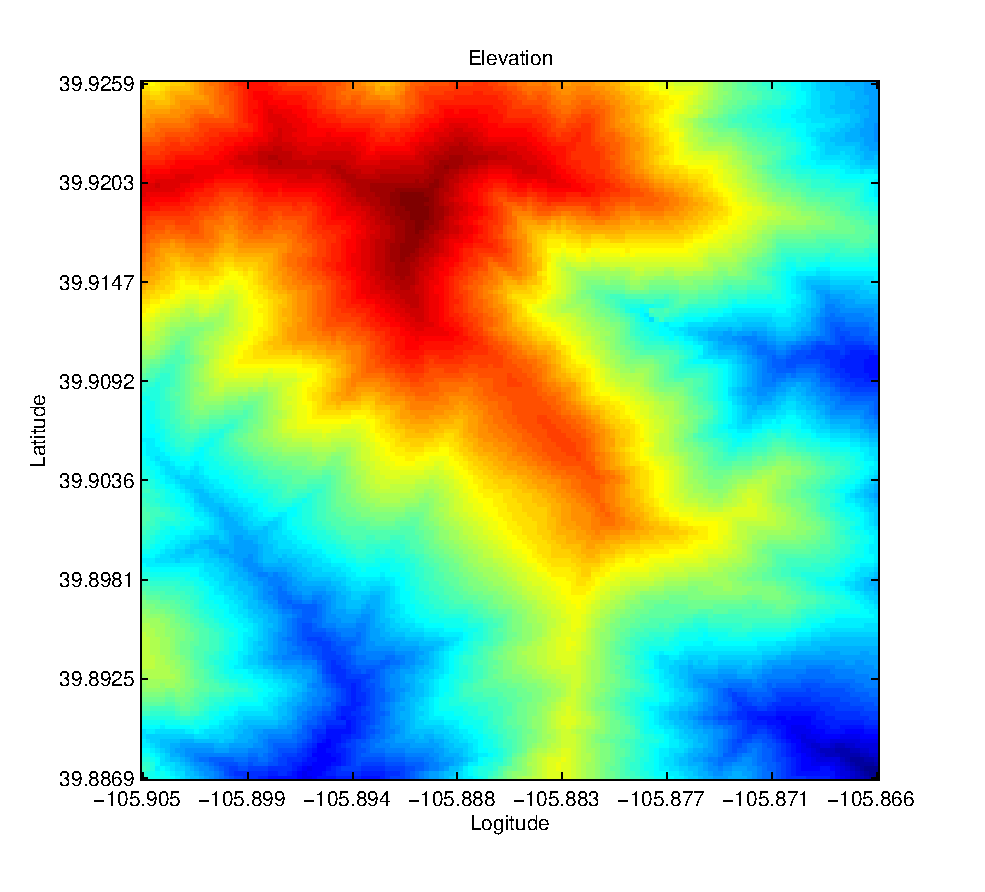
\includegraphics[width=\textwidth]{elev}
	\label{elev}
	\caption{Elevation, red areas indicating higher elevation. Varying elevation effects local wind speed and direction, atmospheric pressure at the surface and sunlight intensity. All of these phenomena effect snow energy flux and sublimation rates. In this model, wind, precipitation and radiation are spatially uniform. This means that atmospheric pressure is likely to be the most significant result of varying elevation. Slope also affects the likelihood of snow accumulation.}
\end{figure}
\begin{figure}
	\includegraphics[width=\textwidth]{slope}
	\label{slope}
	\caption{Slope, red areas indicating higher slope. Together, slope and aspect represent the angle of orientation of the surface. When liquid water is present, slope and aspect largely determine the velocity of runoff. 
Slope and aspect also determine the average solar incidence angle which effects the intensity of solar radiation.}
\end{figure}
\begin{figure}
	\includegraphics[width=\textwidth]{aspect}
	\label{aspect}
	\caption{Aspect. Color indicates the direction of steepest decent.}
\end{figure}

\subsection{(e)}
The initial conditions are spatially uniform are 50 mm SWE and 262 $^\circ$K.
\begin{verbatim}
SWE(:,1)=50.*ones(N_pix,1)     %  millimeters
Tsnow(:,1)=262.*ones(N_pix,1)   % deg. K
\end{verbatim}

\subsection{(f)}
Figures \ref{swe} and \ref{tsnow} depict the SWE and snow temperature for the last day of the model. Table \ref{stats} lists the spatially averaged mean and variance of the model on the last day.
\begin{table}
	\begin{tabular}{rll}
		& SWE & T$_{snow}$ \\
		\midrule
		Mean & 69.5 mm & 258.0  $^\circ$K\\
	Variance & 1.6 mm & 44.5 $^\circ$K
	\end{tabular}
	\caption{Moments for last state variable}
	\label{stats}
\end{table}
\begin{figure}
	\includegraphics[width=\textwidth]{swe}
	\caption{Snow Water Equivalent}
	\label{swe}
\end{figure}
\begin{figure}
	\includegraphics[width=\textwidth]{tsnow}
	\caption{Snow Temperature}
	\label{tsnow}
\end{figure}
\subsection{(g)}
\begin{figure}
	\includegraphics[width=\textwidth]{graph}
	\caption{High, low, and average SWE values over time.}

\end{figure}

\section{2. Review of Univariate PDFs}
\begin{table*}[h]
	\begin{tabular}{rllll}
	Distribution & PDF $f_X(x)$ & Support & Parameters & Notation \\
	\midrule
	Normal Gaussian
	& $\frac{1}{\sqrt{2 \, \pi} \, \sigma} 
	\exp \left[ -\frac{1}{2} \left( \frac{x - \mu}{\sigma} \right)^2 \right]$
	& $x\in(-\infty,\infty)$
	& $\mu \in (-\infty,\infty),\ \sigma>0$
	& $X\sim\mathcal{N}(\mu,\sigma^2)$ \\
	Lognormal 
	& $\frac{1}{\sqrt{2 \, \pi} \, \sigma \, x}
	\exp \left(-\frac{[\ln(x) - \mu]^2}{2 \, \sigma^2} \right)$
	& $x\in(0,\infty)$
	& $\mu \in (-\infty,\infty),\ \sigma>0$
	& $X\sim\ln\mathcal{N}(\mu,\sigma^2)$ \\
	Gamma \footnotemark
	& $\frac{1}{\Gamma(k) \, b^k} x^{k-1} e^{-x/b}$ 
	& $x\in(0,\infty)$
	& $k,b\in(0,\infty)$
	& $X\sim\Gamma(k,b)$ \\
	Beta \footnotemark
	& $\frac{1}{B(a, b)} x^{a-1} (1 - x)^{b-1}$
	& $x\in[0,1]$
	& $a,b\in(0,\infty)$ 
	& $X\sim\text{Beta}(a,b)$ \\
	Exponential
	& $r \, e^{-r\,x}$
	& $x\in[0,\infty)$
	& $r\in(0,\infty)$
	& $X\sim\text{Exp}(r)$
\end{tabular}
\end{table*}
\vspace{3\baselineskip}
\footnotetext[1]{where $\Gamma(k) = \int_0^\infty s^{k-1} e^{-s}\ ds$}
\footnotetext{where $B(a, b) = \int_0^1 u^{a-1} (1 - u)^{b - 1}\ du$}
%\vspace{-7\baselineskip}\footnotetext{test}

\section{3. Review of Univariate PDFs}
\subsection{(a)}
For CDF
\[
	P_X(x)=\left\{
		\begin{array}{l@{\quad\text{for }}r}
			1-\left(\frac{25}{x}\right)^4 & x\geq25 \\
			0 & x<25
		\end{array}
		\right.
		\quad \text{(cm)}
	\] 
the PDF is
\[
	p_X(x)=\left\{
		\begin{array}{l@{\quad\text{for }}r}
			\frac{dP_X}{dx} & \geq25 \\
			0 & x<25
		\end{array}
		\right.
	=\left\{
		\begin{array}{l@{\quad\text{for }}r}
			4(25^4) x^{-5} & x\geq25 \\
			0 & x<25
		\end{array}
		\right.
		\quad \text{(cm)}
	\]

\subsection{(b)}
\[
	\E X = \int_{-\infty}^\infty xp_X(x)\ dx = 0 + \int_{25}^\infty 4x(25^4) x^{-5} \approx 33.33 \text{ cm}
\]
\subsection{(c)}
\[
	\text{Pr}(27 \text{ cm}< x \leq 32\text{ cm}) = P_X(32\text{ cm}) - P_X(27\text{ cm}) \approx 0.363 
\]
\subsection{(d)}
\[
	\text{Pr}(x > 35\text{ cm}) = 1-\text{Pr}(x \leq 35\text{ cm}) = 1-P_X(35\text{ cm})\approx 0.260 
\]

\end{document}
